\documentclass[tikz,border=4pt]{standalone}
% Estilo común de los diagramas de bloques (se usa con \input en cada standalone)
\usepackage[defaultsans,scale=0.92]{lato}
\usepackage{libertinust1math}
\usepackage{xcolor,amsmath}
\usepackage{tikz}
\usetikzlibrary{positioning,arrows.meta,calc,shapes.geometric}
\usepackage{../../notacion}
\definecolor{ctrlazul}{HTML}{1E5AA8}\definecolor{ctrlnoche}{HTML}{14213D}
\definecolor{ctrlcoral}{HTML}{D1495B}\definecolor{ctrlverde}{HTML}{2A9D8F}
\definecolor{ctrlambar}{HTML}{E09F3E}\definecolor{ctrlgris}{HTML}{5C677D}
\definecolor{ctrlvioleta}{HTML}{6C4AB6}\definecolor{ctrlteal}{HTML}{0F7173}
\tikzset{
  >={Stealth[length=2.4mm]}, every node/.style={font=\small},
  bloque/.style={draw=ctrlnoche,fill=ctrlazul!7,thick,rounded corners=1.5pt,minimum height=9mm,minimum width=13mm,inner sep=4pt},
  suma/.style={draw=ctrlnoche,thick,circle,inner sep=0pt,minimum size=6mm},
  senal/.style={->,thick,draw=ctrlnoche},
  rot/.style={font=\footnotesize,text=ctrlgris},
}

\begin{document}
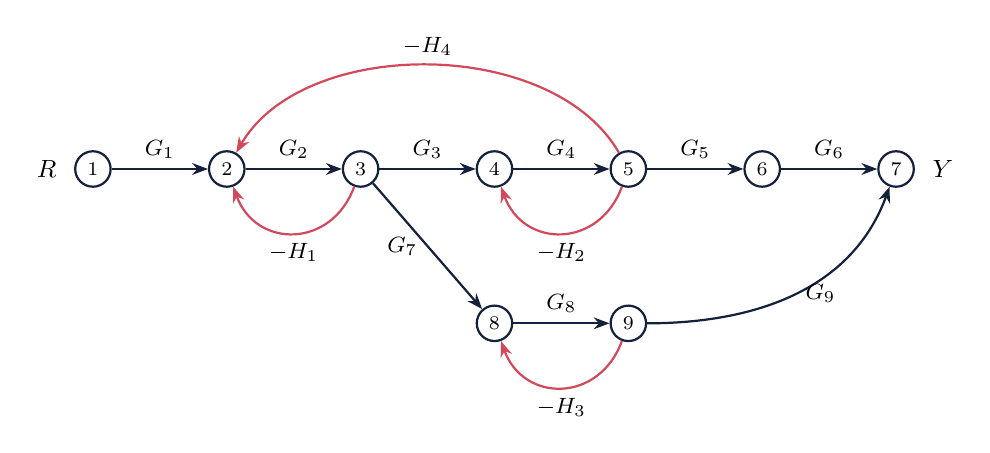
\begin{tikzpicture}[x=17mm,y=14mm,
  nodo/.style={circle,draw=ctrlnoche,thick,fill=white,minimum size=4.5mm,inner sep=0pt,font=\scriptsize},
  rama/.style={-{Stealth[length=2mm]},thick,draw=ctrlnoche},
  ret/.style={-{Stealth[length=2mm]},thick,draw=ctrlcoral},
  et/.style={font=\footnotesize}]
  \foreach \i/\x/\y in {1/0/0,2/1/0,3/2/0,4/3/0,5/4/0,6/5/0,7/6/0,8/3/-1.4,9/4/-1.4}
     \node[nodo] (n\i) at (\x,\y) {\i};
  \node[left=1mm of n1] {$R$}; \node[right=1mm of n7] {$Y$};
  \draw[rama] (n1)--node[above,et]{$G_1$}(n2);
  \draw[rama] (n2)--node[above,et]{$G_2$}(n3);
  \draw[rama] (n3)--node[above,et]{$G_3$}(n4);
  \draw[rama] (n4)--node[above,et]{$G_4$}(n5);
  \draw[rama] (n5)--node[above,et]{$G_5$}(n6);
  \draw[rama] (n6)--node[above,et]{$G_6$}(n7);
  \draw[rama] (n3)--node[left,et]{$G_7$}(n8);
  \draw[rama] (n8)--node[above,et]{$G_8$}(n9);
  \draw[rama] (n9) to[out=0,in=-110] node[right,et]{$G_9$}(n7);
  \draw[ret] (n3) to[out=-110,in=-70,looseness=1.4] node[below,et]{$-H_1$}(n2);
  \draw[ret] (n5) to[out=-110,in=-70,looseness=1.4] node[below,et]{$-H_2$}(n4);
  \draw[ret] (n9) to[out=-110,in=-70,looseness=1.4] node[below,et]{$-H_3$}(n8);
  \draw[ret] (n5) to[out=120,in=60,looseness=0.9] node[above,et]{$-H_4$}(n2);
\end{tikzpicture}
\end{document}
